% !TeX root = ../../Skript.tex
\cohead{\Large\textbf{Wurzeln}}
\fakesubsection{Wurzeln}
\setlength{\qrheight}{2.5cm}%
\newlength{\wurzelnLength}%
\iftoggle{qrcode}{\setlength{\wurzelnLength}{\textwidth-\qrheight}}{\setlength{\wurzelnLength}{\textwidth}}%
\begin{minipage}{\textwidth}
    \adjustbox{valign=t}{\begin{minipage}{\wurzelnLength}
            Wir werden Wurzeln zum Lösen von Gleichungen vom Typ \mbox{\(x^n=y\)} verwenden, wobei die Hochzahl \(n=2,\ 3,\ 4,\dots\) eine natürliche Zahl größer gleich 2 ist. Die uns bekannte Wurzel ist eigentlich die zweite Wurzel \mbox{\(\sqrt[\leftroot{0}\uproot{1}2]{y}  =\sqrt{y}\)}. Für jede der möglichen Hochzahlen \mbox{\(2,\ 3,\ 4,\dots\)} ist eine eigene Wurzel definiert, z.B. \(\sqrt[\leftroot{0}\uproot{1}3]{y}\). Grob vereinfacht macht die \(n\)-te Wurzel das hoch \(n\) rückgängig bzw. kehrt es um. Etwas anschaulicher sucht die \(n\)-te Wurzel zu einem gegebenen \(y\)-Wert den passenden \(x\)-Wert im Schaubild von \(x^n\):
    \end{minipage}}%
    \iftoggle{qrcode}{%
        \adjustbox{valign=t}{\begin{minipage}{\qrheight}
                \href{https://www.geogebra.org/m/sgznd756}{
\includegraphics[height=\qrheight]{\ganzFkt/pics/WurzelnQR.png}}%
        \end{minipage}}%
    }{}%
\end{minipage}

\medskip

\textbf{Gerade Wurzeln}

\smallskip

\begin{minipage}{\textwidth}
	\adjustbox{valign=t}{\begin{minipage}{0.4\textwidth}
			\centering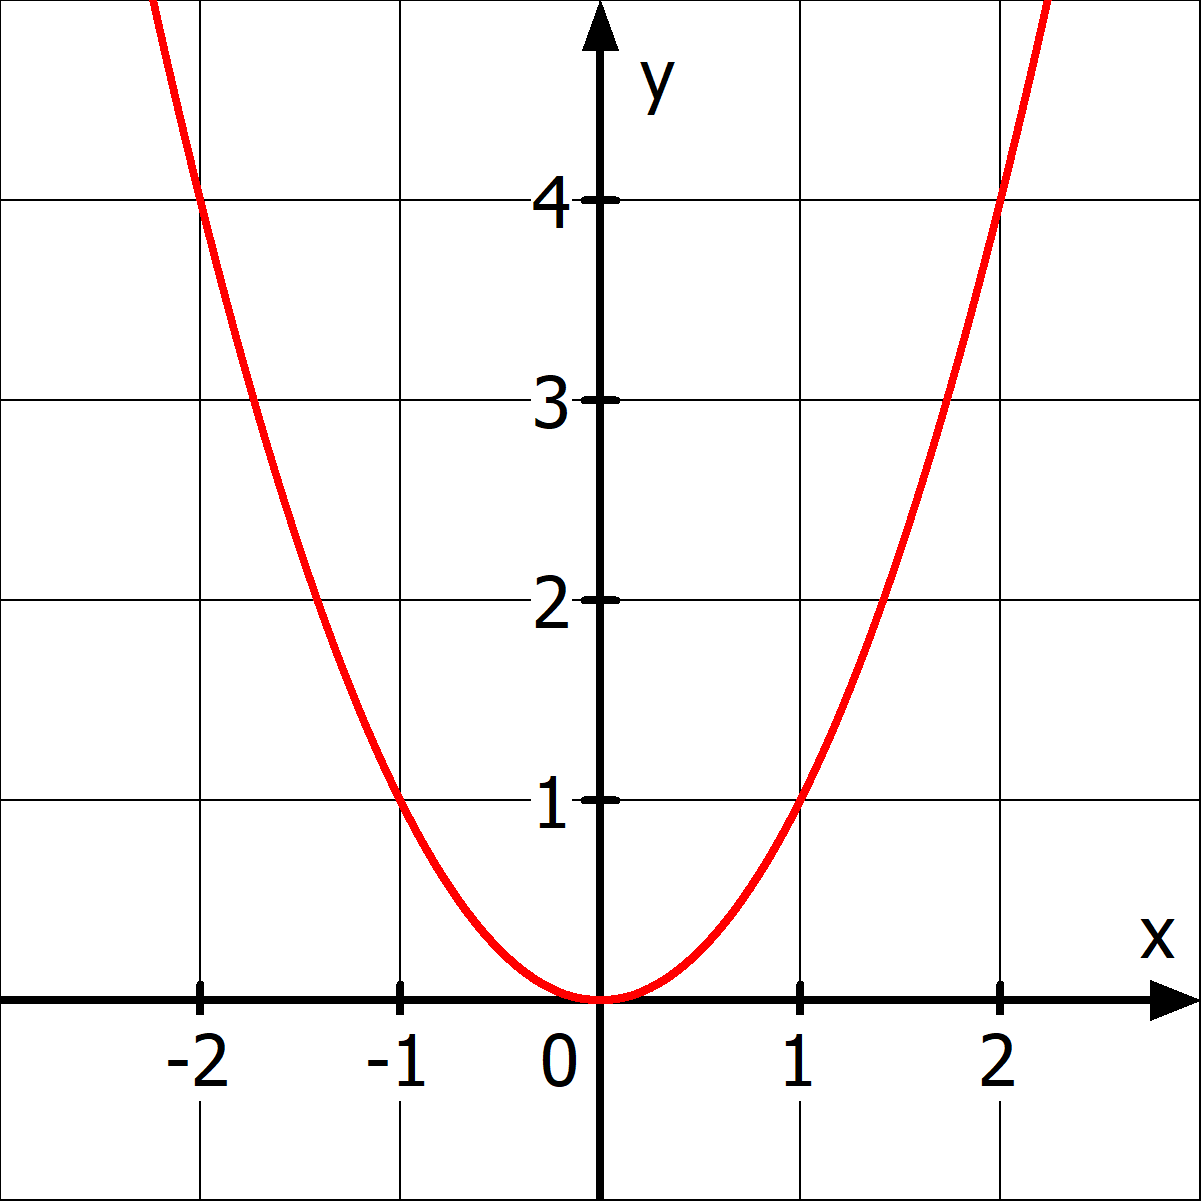
\includegraphics[width=\textwidth]{\ableitung/pics/geradeWurzel.png}
	\end{minipage}}%
	\adjustbox{valign=t, padding =1ex 0ex 0ex 0ex}{\begin{minipage}{0.6\textwidth-1ex}\raggedright
			\textcolor{loes}{Die Schaubilder von \(x^n\) für gerade \(n\) sind alle parabelförmig, daher verhalten sich auch ihre \mbox{\(n\)-ten} Wurzeln alle ähnlich. Zu jedem positiven \mbox{\(y\)-Wert} gibt es zwei mögliche \mbox{\(x\)-Werte}, z.B. gibt es zum \mbox{\(y\)-Wert} 4 die beiden möglichen \mbox{\(x\)-Werte} 2 und -2, daher gilt \mbox{\(\sqrt{4}=\pm2\)}.}%

			\textcolor{loes}{Zum \mbox{\(y\)}-Wert 0 gibt es nur den \mbox{\(x\)}-Wert 0: \mbox{\(\sqrt{0}=0\)}.}%

			\textcolor{loes}{Zu einem negativen \mbox{\(y\)-Wert} gibt es keinen passenden \mbox{\(x\)-Wert}, da die Schaubilder von \(x^n\) keine negativen \mbox{\(y\)-Werte} haben, daher darf man unter gerade Wurzeln keine negativen Zahlen einsetzen, bzw. die gerade Wurzel einer negativen Zahl ist nicht definiert, z.B. \mbox{\(\sqrt{-0,5}\)\Lightning}.}%
	\end{minipage}}%
\end{minipage}

\bigskip

\textbf{Ungerade Wurzeln}

\smallskip

\begin{minipage}{\textwidth}
	\adjustbox{valign=t, padding =0ex 1ex 0ex 0ex}{\begin{minipage}{0.6\textwidth}\raggedright
			\textcolor{loes}{Die Schaubilder von \(x^n\) für ungerade \(n\) sind alle S-förmig. Zu jedem \mbox{\(y\)-Wert} gibt es nun genau einen passenden \mbox{\(x\)-Wert}, d.h. man darf alle Zahlen unter die Wurzel schreiben und erhält immer genau eine Lösung:}

			\textcolor{loes}{\(\sqrt[\leftroot{0}\uproot{1}3]{1}=1\), aber -1 ist keine Lösung, da \((-1)^3=-1\neq1\).}

			\textcolor{loes}{Dafür gilt \(\sqrt[\leftroot{0}\uproot{1}3]{-1}=-1\).}
	\end{minipage}}%
	\adjustbox{valign=t}{\begin{minipage}{0.4\textwidth}
			\centering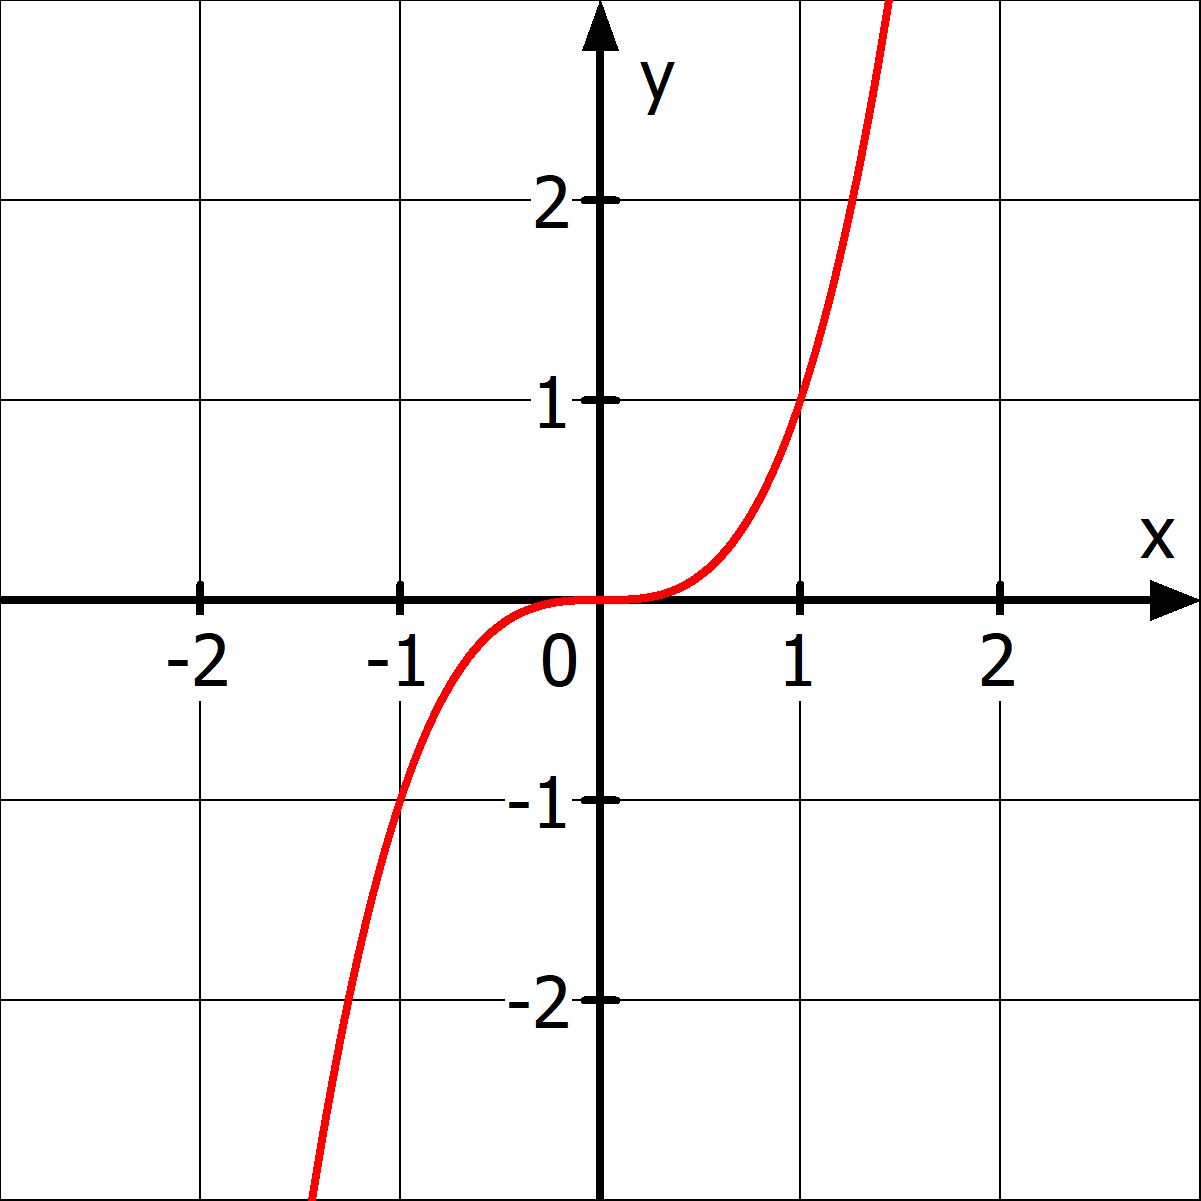
\includegraphics[width=\textwidth]{\ableitung/pics/ungeradeWurzel.png}
	\end{minipage}}%
\end{minipage}

\begin{itemize}
	\item[\textcolor{loes}{\textbullet}] \textcolor{loes}{Gerade Wurzeln}\\
	\textcolor{loes}{Nur positive Zahlen unter die Wurzel, dafür 2 Lösungen:}\\
	\textcolor{loes}{\(\sqrt[\leftroot{0}\uproot{1}n]{\text{positive Zahl}}=\pm\text{Lösung}\)}\\
	\textcolor{loes}{\(\sqrt[\leftroot{0}\uproot{1}n]{\text{negative Zahl}}\text{ keine Lösung}\)\Lightning}
	\item[\textcolor{loes}{\textbullet}] \textcolor{loes}{Ungerade Wurzeln}\\
	\textcolor{loes}{Jede Zahl darf unter die Wurzel geschrieben werden, immer genau 1 Lösung:}\\
	\textcolor{loes}{\(\sqrt[\leftroot{0}\uproot{1}n]{\text{positive Zahl}}=\text{1 Lösung (positiv)}\)}\\
	\textcolor{loes}{\(\sqrt[\leftroot{0}\uproot{1}n]{\text{negative Zahl}}=\text{1 Lösung (negativ)}\)}
\end{itemize}